% Week 4: Convolutional Neural Networks I
\chapter{Week 4: Convolutional Neural Networks I}
\label{ch:week4}

% ============================================================================
% CHAPTER INTRODUCTION - Intuitive framing before any formalism
% ============================================================================

Imagine trying to describe what makes a cat recognisable. You might mention pointy ears, whiskers, a particular nose shape, and perhaps distinctive eyes. Notice that you naturally describe \emph{local features}-small, characteristic patterns-rather than listing the colour of every pixel. This intuition lies at the heart of Convolutional Neural Networks (CNNs): instead of treating an image as a flat list of unrelated pixel values, CNNs systematically scan for meaningful local patterns and build up increasingly complex features from simple ones.

This chapter introduces the fundamental building blocks of CNNs. We will see how a simple operation-sliding a small ``template'' across an image and measuring similarity-can be stacked to create systems that rival human visual perception. The key insights are:

\begin{enumerate}
    \item \textbf{Locality matters}: Nearby pixels are far more related than distant ones. A pixel in a cat's ear tells you much more about the surrounding ear pixels than about pixels in the background.

    \item \textbf{Features repeat}: A vertical edge is a vertical edge, whether it appears in the top-left or bottom-right of an image. We should not need to learn separate ``edge detectors'' for every possible position.

    \item \textbf{Hierarchy emerges}: Simple features (edges, colours) combine into textures, textures combine into parts (eyes, wheels), and parts combine into objects (cats, cars). This hierarchical composition happens automatically through training.
\end{enumerate}

\begin{quickref}[Chapter Overview]
\textbf{Core goal:} Understand how convolutional neural networks exploit spatial structure for efficient image processing.

\textbf{Key topics:}
\begin{itemize}
    \item Why CNNs? Challenges with fully connected layers for images
    \item Convolution and cross-correlation operations (full mathematical treatment)
    \item Padding strategies, stride, and output dimensions
    \item Pooling for dimensionality reduction and translation invariance
    \item Multi-channel inputs and outputs
    \item Backpropagation through convolutional layers
    \item Translation equivariance vs invariance
    \item Receptive fields and architecture design principles
\end{itemize}

\textbf{Key equations:}
\begin{itemize}
    \item Cross-correlation: $(X \star W)_{ij} = \sum_{p,q} x_{i+p, j+q} \cdot w_{p,q}$
    \item Output dimension: $\left\lfloor \frac{d + 2P - r}{S} \right\rfloor + 1$
    \item Receptive field: $\text{RF}_l = \text{RF}_{l-1} + (r_l - 1) \cdot \prod_{i=1}^{l-1} s_i$
    \item Conv gradient: $\frac{\partial L}{\partial W} = X \star \delta$ (rotated cross-correlation)
\end{itemize}
\end{quickref}

\textbf{Prerequisites:} This chapter assumes familiarity with basic neural network concepts (layers, activations, backpropagation) and matrix operations. If terms like ``gradient descent'' or ``activation function'' are unfamiliar, review the earlier chapters on neural network fundamentals first.

%==============================================================================
\section{Computer Vision Tasks}
%==============================================================================

Before diving into how CNNs work, let us establish \emph{what} we want them to do. Computer vision-teaching machines to interpret visual information-encompasses several distinct tasks, each requiring different levels of understanding.

Think of these tasks as answering increasingly specific questions about an image:
\begin{itemize}
    \item \textbf{Classification}: ``What is in this image?'' (one answer for the whole image)
    \item \textbf{Detection}: ``What objects are present, and where are they?'' (bounding boxes)
    \item \textbf{Segmentation}: ``Which pixels belong to which object?'' (pixel-level labels)
\end{itemize}

\begin{figure}[H]
    \centering
    \includegraphics[width=1\linewidth]{images/week_4/Screenshot 2024-10-22 at 17.49.34.png}
    \caption{Common computer vision tasks: classification assigns one label to the whole image; detection locates objects with bounding boxes; segmentation classifies every pixel. Each task provides progressively more detailed information about the image content.}
    \label{fig:cv-tasks}
\end{figure}

Computer vision encompasses a hierarchy of tasks with increasing complexity and granularity of output:

\begin{rigour}[Computer Vision Task Hierarchy]
\begin{enumerate}
    \item \textbf{Image classification}: Assign a single label to the entire image
    \begin{itemize}
        \item Input: Image $X \in \mathbb{R}^{H \times W \times C}$
        \item Output: Class probability vector $\hat{y} \in \mathbb{R}^K$
        \item Example: ``This image contains a cat'' (probability 0.95)
        \item \textit{Note on notation:} $H$ is height (rows), $W$ is width (columns), $C$ is channels (e.g., 3 for RGB), and $K$ is the number of possible classes
    \end{itemize}

    \item \textbf{Object detection}: Locate and classify multiple objects
    \begin{itemize}
        \item Output: Set of bounding boxes with class labels $\{(x, y, w, h, c)_i\}$
        \item Each detection specifies: position $(x, y)$, size $(w, h)$, and class $c$
        \item Example: ``Cat at position (100, 150) with size 200$\times$180''
    \end{itemize}

    \item \textbf{Semantic segmentation}: Classify every pixel
    \begin{itemize}
        \item Output: Per-pixel class labels $Y \in \{1, \ldots, K\}^{H \times W}$
        \item Every pixel gets a class label, but different cats are not distinguished
        \item Example: ``Pixels (100--200, 150--300) are cat; (0--50, 0--100) are sky''
    \end{itemize}

    \item \textbf{Instance segmentation}: Distinguish individual object instances
    \begin{itemize}
        \item Output: Per-pixel labels with instance IDs
        \item Combines semantic segmentation with instance identification
        \item Example: ``Pixels (100--200, 150--300) are Cat \#1; (400--500, 200--350) are Cat \#2''
    \end{itemize}
\end{enumerate}
\end{rigour}

Each task builds on the capabilities needed for simpler tasks. A network that can segment objects typically incorporates the feature extraction abilities of a classifier, extended with spatial precision. This chapter focuses primarily on the foundational architecture for \textbf{classification}, which provides the building blocks for all other tasks.

\subsection{Human vs Computer Perception}

To appreciate why CNNs were designed the way they are, we must first understand the chasm between human and machine perception of images.

When you look at a photograph of a dog, you instantly recognise it as a dog. You do not consciously process the millions of individual pixel values; instead, your visual system automatically extracts meaningful features-the shape of the snout, the texture of fur, the position of eyes and ears-and combines them into the coherent percept ``dog''. Remarkably, you recognise the dog whether it is large or small in the image, whether it is in the corner or the centre, whether the lighting is bright or dim.

A computer, by contrast, sees something entirely different: a large matrix of numbers.

\begin{quickref}[Human vs Machine Vision]
\textbf{Humans:}
\begin{itemize}
    \item Look for local features (edges, textures, shapes)
    \item Automatically ignore irrelevant information (background clutter)
    \item Recognise objects regardless of position, scale, lighting
    \item Process visual information hierarchically (low-level to high-level)
    \item Effortlessly generalise from few examples
\end{itemize}

\textbf{Computers:}
\begin{itemize}
    \item See a matrix of pixel values (typically integers 0--255 for 8-bit images)
    \item Each pixel is just a number with no inherent meaning
    \item Colour images have multiple channels (RGB = 3 channels, one for red, green, blue)
    \item Can also process hyperspectral images (100s of channels beyond visible light)
    \item Require explicit algorithms to extract meaning from raw pixels
\end{itemize}
\end{quickref}

\textbf{What does a computer actually ``see''?} Consider a small $3 \times 3$ grayscale image patch. To a human viewing the rendered image, this might show part of an edge or a corner. To the computer, it is simply:
\[
\begin{bmatrix}
45 & 128 & 200 \\
50 & 130 & 198 \\
48 & 125 & 195
\end{bmatrix}
\]
Nine numbers with no inherent structure. The fact that the left column has low values (dark) and the right column has high values (bright) is not ``known'' to the computer-it must be discovered through processing.

For colour images, each pixel has three values (red, green, blue intensity), so a $224 \times 224$ RGB image is a 3D array of $224 \times 224 \times 3 = 150{,}528$ numbers. The challenge of computer vision is to transform this unstructured pile of numbers into meaningful understanding: ``This is a golden retriever playing fetch in a park.''

Understanding this fundamental difference motivates the design of CNNs: we want to build systems that can learn to extract the same hierarchical, position-invariant features that human vision processes effortlessly. CNNs achieve this through clever architectural choices that encode our prior knowledge about the structure of visual information.

%==============================================================================
\section{Why Convolutional Layers?}
%==============================================================================

Before CNNs became dominant in the 2010s, the standard approach to image processing with neural networks was to use \textbf{fully connected layers}-the same architecture used for tabular data. This section explains why that approach fails catastrophically for images and how convolutional layers solve these problems.

The key insight is that images have \emph{structure} that fully connected layers ignore. Specifically:
\begin{itemize}
    \item Pixels are arranged on a 2D grid, and this arrangement carries meaning
    \item Nearby pixels tend to be correlated (part of the same object or texture)
    \item The same pattern (an edge, a texture) can appear anywhere in the image
\end{itemize}

Convolutional layers are designed from the ground up to exploit this structure.

\begin{quickref}[CNN Motivation]
CNNs address three key challenges that arise when processing images with neural networks:
\begin{enumerate}
    \item \textbf{Reduce parameters}: Weight sharing across spatial locations (the same small filter is reused everywhere)
    \item \textbf{Leverage locality}: Nearby pixels are more related than distant ones (local connectivity)
    \item \textbf{Translation equivariance}: Detect features regardless of position (a vertical edge is a vertical edge, wherever it appears)
\end{enumerate}

Each of these is a \emph{design choice} that encodes our prior knowledge about the structure of images. This ``inductive bias'' makes CNNs far more data-efficient than generic fully connected networks.
\end{quickref}

\subsection{Challenge 1: Spatial Structure}

The first problem with fully connected layers is that they completely ignore the spatial arrangement of pixels. Let us see why this matters.

Fully connected layers destroy spatial relationships in images.

\begin{figure}[H]
    \centering
    \includegraphics[width=0.5\linewidth]{images/week_4/fully connected.png}
    \caption{Fully connected network: every neuron in one layer connects to every neuron in the next. For images, this means flattening the 2D spatial structure into a 1D vector, losing all notion of ``which pixels are neighbours.''}
    \label{fig:fully-connected}
\end{figure}

\textbf{What is a fully connected layer?} In a fully connected (FC) layer, also called a \emph{dense} layer, every output neuron receives input from \emph{every} input neuron. There are no restrictions on connectivity-every possible connection exists.

\begin{rigour}[Fully Connected Layer]
In a fully connected layer, each output neuron $j$ computes a weighted sum of \emph{all} inputs:
\[
h^{[l]}_j = \sigma \left( \sum_{i=1}^{H^{[l-1]}} W^{[l]}_{ji} h^{[l-1]}_i + b^{[l]}_j \right)
\]

Let us unpack this equation term by term:
\begin{itemize}
    \item $h^{[l]}_j$ is the activation (output) of neuron $j$ in layer $l$
    \item $h^{[l-1]}_i$ is the activation of neuron $i$ in the previous layer $(l-1)$
    \item $W^{[l]}_{ji}$ is the weight connecting input $i$ to output $j$ (note: $j$ indexes the output, $i$ indexes the input)
    \item $b^{[l]}_j$ is the bias term for output neuron $j$
    \item $\sigma(\cdot)$ is a non-linear activation function (e.g., ReLU, sigmoid)
    \item The sum runs over \textbf{all} $H^{[l-1]}$ neurons in the previous layer
\end{itemize}

\textbf{Problem for images:}
\begin{itemize}
    \item Images must be \textbf{flattened} to a 1D vector before input (a $28 \times 28$ image becomes a 784-element vector)
    \item Spatial relationships between pixels are completely lost-pixel $(0, 0)$ is no longer ``next to'' pixel $(0, 1)$
    \item Each pixel is treated as an independent input feature-there is no notion of ``nearby''
    \item The network must learn that pixel $(0, 1)$ is related to pixel $(0, 0)$ from scratch, for every position in the image
\end{itemize}
\end{rigour}

To make this concrete, consider what happens when we flatten a $3 \times 3$ image patch:
\[
\begin{bmatrix}
a & b & c \\
d & e & f \\
g & h & i
\end{bmatrix}
\xrightarrow{\text{flatten}}
[a, b, c, d, e, f, g, h, i]
\]
In the original image, pixel $b$ is adjacent to $a$, $c$, and $e$. After flattening, $b$ is adjacent only to $a$ and $c$ in the vector, and its relationship to $e$ (directly below it) is completely lost. A fully connected layer sees no difference between the relationship of $b$ to $e$ (one row apart in the image) and $b$ to $g$ (two rows apart).

\begin{redbox}
\textbf{Nearby pixels are related!} Flattening an image discards critical spatial information. In natural images, a pixel's neighbours contain much more relevant information than distant pixels-they are likely part of the same object, texture, or edge. But fully connected layers treat all inputs equally, giving a pixel in the top-left corner the same opportunity to influence an output as its immediate neighbour. This violates the \textbf{locality principle} that underlies much of visual perception.

\textbf{Analogy}: Imagine trying to recognise a friend's face from a shuffled list of their facial feature colours. You have all the information, but the structure that makes a face recognisable is destroyed.
\end{redbox}

\subsection{Challenge 2: Parameter Explosion}

The second devastating problem with fully connected layers is the sheer number of parameters required. Each connection between neurons requires one weight parameter, and the number of connections grows as the \emph{product} of input and output sizes.

\textbf{Why does this matter?} More parameters means:
\begin{enumerate}
    \item More memory to store the weights (both during training and inference)
    \item More computation to perform the matrix multiplications
    \item More training data needed to learn meaningful patterns (rather than memorising)
    \item Higher risk of overfitting (the model memorises training examples instead of learning generalisable features)
\end{enumerate}

\begin{rigour}[Parameter Count Problem]
For a fully connected layer, the number of parameters is:
\[
\text{Parameters} = (\text{input size}) \times (\text{output size}) + (\text{output size})
\]
The first term accounts for the weights; the second for the biases (one per output neuron).

\textbf{Example 1}: A modest 1 megapixel RGB image ($1000 \times 1000 \times 3 = 3 \times 10^6$ values) connected to just 1000 hidden units:
\[
\text{Parameters} = 3 \times 10^6 \times 10^3 + 10^3 \approx 3 \times 10^9
\]

\textbf{Three billion parameters} for a single layer!

\textbf{What does this mean in practice?}
\begin{itemize}
    \item \textbf{Memory}: Each parameter stored as a 32-bit float takes 4 bytes. Three billion parameters require $3 \times 10^9 \times 4 = 12$ GB just for the weights of one layer
    \item \textbf{Computation}: A single forward pass through this layer requires $3 \times 10^9$ multiply-add operations
    \item \textbf{Overfitting}: The ImageNet training set has about 1.2 million images. With 3 billion parameters, the network could memorise $\approx 2500$ values per training image-far more than needed to simply store the correct label
\end{itemize}
\end{rigour}

\textbf{Example 2}: Even for the ``small'' MNIST dataset ($28 \times 28 = 784$ pixels, grayscale), connecting to 1000 hidden units requires $784 \times 1000 = 784{,}000$ parameters. With only 60,000 training images, that is about 13 parameters per training pixel-a recipe for overfitting.

\begin{quickref}[Parameter Comparison]
For a $224 \times 224 \times 3$ image (standard ImageNet input size):
\begin{itemize}
    \item \textbf{Fully connected} to 4096 units: $224 \times 224 \times 3 \times 4096 = 616{,}562{,}688 \approx 617$ million parameters
    \item \textbf{Convolutional layer} with 64 filters of $3 \times 3$: $3 \times 3 \times 3 \times 64 + 64 = 1{,}792$ parameters
\end{itemize}
A reduction factor of $\approx 350{,}000\times$!

The convolutional layer achieves this dramatic reduction through two mechanisms:
\begin{enumerate}
    \item \textbf{Local connectivity}: Each output depends only on a small $3 \times 3$ region, not the entire image
    \item \textbf{Weight sharing}: The same 27 weights (plus bias) are reused at every spatial position
\end{enumerate}
\end{quickref}

\subsection{Challenge 3: Translation Invariance}

The third problem is subtle but crucial: for many tasks, we care about \textit{what} is present in an image, not \textit{where} exactly it appears.

Consider a cat classifier. If someone takes a photo of a cat sitting on the left side of the frame, it is still a cat. If they take another photo with the cat on the right, it is still the same cat. The classifier should give the same answer-``cat''-regardless of where the cat appears in the image.

With a fully connected layer, this is a disaster. The weights connecting to ``cat-detector'' neurons are tied to specific pixel positions. A weight that has learned to detect a cat's ear in the top-left must be duplicated (and somehow coordinated with) weights detecting cat ears everywhere else in the image. The network must essentially learn \emph{separate} cat detectors for every possible position-an enormous waste of capacity.

What we want is a system where the same ``cat ear detector'' is applied everywhere, automatically.

\begin{rigour}[Translation Invariance vs Equivariance]
Let $T_\tau$ denote a translation operator that shifts an image by offset $\tau$ (moving all pixels by $\tau$ positions), and let $f$ be a function (e.g., a neural network layer).

\textbf{Translation invariance:}
\[
f(T_\tau[X]) = f(X) \quad \forall \tau
\]
The output is \textbf{unchanged} regardless of where a feature appears. Shifting the input has no effect on the output.

\textbf{Translation equivariance:}
\[
f(T_\tau[X]) = T_\tau[f(X)] \quad \forall \tau
\]
If the input shifts, the output shifts by the \textbf{same amount}. The transformation ``commutes'' with the function.

\textbf{Key distinction:}
\begin{itemize}
    \item \textbf{Invariance}: The output is a fixed value (or vector) that does not change with translation. Useful for final classification: ``This is a cat.''
    \item \textbf{Equivariance}: The output is a spatial map that shifts along with the input. Useful for intermediate representations: ``There is an edge \emph{here}, and it moves if the input moves.''
\end{itemize}
\end{rigour}

\begin{quickref}[Translation Invariance vs Equivariance]
\textbf{Translation invariance:} Output is the same regardless of where a feature appears.
\begin{itemize}
    \item Question: ``Is there a cat?'' $\rightarrow$ Answer: Yes/No (position does not matter)
    \item Achieved through pooling operations and global aggregation
    \item Desired for classification tasks
\end{itemize}

\textbf{Translation equivariance:} If input shifts, output shifts by the same amount.
\begin{itemize}
    \item Question: ``Where are the edges?'' $\rightarrow$ Answer: A map showing edge locations (map shifts if image shifts)
    \item Convolutions are naturally equivariant
    \item Desired for intermediate feature maps (we want to know \emph{where} features are, even if we later discard location)
\end{itemize}
\end{quickref}

\textbf{Why do we want both?} CNNs are designed to build \emph{equivariant} intermediate representations that progressively aggregate into \emph{invariant} final outputs:
\begin{enumerate}
    \item Early layers use convolution (equivariant): edge detectors that activate wherever edges appear
    \item Pooling gradually introduces local invariance: aggregating nearby responses
    \item Final layers (global pooling or fully connected) achieve full invariance: ``Is there a cat?''
\end{enumerate}

This combination allows CNNs to detect features anywhere in the image (through equivariance) while ultimately producing position-independent classifications (through invariance).

%==============================================================================
\section{Properties of CNNs}
%==============================================================================

Now that we understand the problems with fully connected layers for images, let us examine how convolutional layers solve them. The key properties of CNNs are not arbitrary design choices-each directly addresses one of the challenges we identified.

\begin{rigour}[CNN Key Properties]
\begin{enumerate}
    \item \textbf{Local connectivity (sparse interactions)}: Each output unit depends only on a small local region of the input, called the \textit{receptive field}

    \textit{How it helps:} Exploits the locality of natural images (nearby pixels are correlated). Dramatically reduces parameters since each output connects to only $r \times r$ inputs instead of all inputs.

    \item \textbf{Weight sharing (parameter tying)}: The same filter weights are applied at every spatial location-the filter is ``slid'' across the image

    \textit{How it helps:} Further reduces parameters (one set of weights for all positions). Encodes the assumption that a feature worth detecting in one location is worth detecting everywhere.

    \item \textbf{Translation equivariance}: A consequence of weight sharing; if the input pattern shifts, the feature map shifts identically

    \textit{How it helps:} The network need not learn separate detectors for each position. A single ``vertical edge detector'' works across the entire image.

    \item \textbf{Hierarchical features}: Stacking layers allows detection of increasingly complex patterns

    \textit{How it helps:} Edges combine into textures, textures into parts, parts into objects. This compositional structure matches how visual information is naturally organised.
\end{enumerate}
\end{rigour}

Let us unpack each property in more detail.

\textbf{Local connectivity} means that a neuron in a convolutional layer does not ``see'' the entire input image. Instead, it sees only a small patch-typically $3 \times 3$, $5 \times 5$, or $7 \times 7$ pixels. This patch is the neuron's \emph{receptive field}. The assumption is that useful features are local: an edge can be detected from a small neighbourhood without needing information from the opposite corner of the image.

\textbf{Weight sharing} means that the same small set of weights is used at every position. Imagine sliding a $3 \times 3$ template across the image, computing a dot product at each location. The template has only 9 weights, regardless of whether the image is $28 \times 28$ or $1000 \times 1000$. This is in stark contrast to fully connected layers, where each position has its own weights.

\textbf{Translation equivariance} is a direct consequence of weight sharing. Since the same weights are used everywhere, shifting the input simply shifts the output. If a vertical edge appears at position $(10, 20)$ and the ``edge detector'' filter responds strongly there, then shifting the edge to position $(15, 25)$ will shift the response to $(15, 25)$ as well.

\textbf{Hierarchical features} emerge from stacking convolutional layers. The first layer sees raw pixels and learns to detect simple features like edges and colour gradients. The second layer sees the output of the first layer and learns to detect combinations of edges-corners, junctions, simple textures. Deeper layers see increasingly abstract combinations, eventually representing high-level concepts like ``eye'' or ``wheel.''

\begin{quickref}[CNN Advantages]
\begin{itemize}
    \item \textbf{Fewer parameters}: Weight sharing reduces a potential $10^9$ parameters to $10^3$ for typical layers
    \item \textbf{Parallelisable}: Convolutions at different spatial locations are independent and can be computed simultaneously
    \item \textbf{GPU-friendly}: Convolutions can be expressed as matrix multiplications (via im2col), which GPUs excel at
    \item \textbf{Robust to position}: The same filter detects patterns anywhere in the image
    \item \textbf{Robust to illumination}: Filters detect relative patterns (edges are defined by intensity \emph{differences}) regardless of absolute brightness
    \item \textbf{Data efficient}: The inductive biases (locality, translation equivariance) mean less training data is needed to learn good representations
\end{itemize}
\end{quickref}

\subsection{Intuitive Summary: What Convolution Does}

Before diving into the mathematics, here is an intuitive summary of what convolution achieves:

\begin{itemize}
    \item A \textbf{filter} (or \textbf{kernel}) is a small template, typically $3 \times 3$ or $5 \times 5$ pixels, containing learnable weights
    \item The filter is \textbf{slid} across the image, one position at a time
    \item At each position, we compute a \textbf{weighted sum} (essentially a dot product) between the filter and the image patch it overlays
    \item High output = the patch looks like the filter; low/negative output = it does not
    \item The collection of outputs at all positions forms a \textbf{feature map} (or \textbf{activation map})
    \item Different filters detect different features: one might respond to vertical edges, another to horizontal edges, another to specific colour combinations
\end{itemize}

Think of it as systematically asking ``Does this part of the image look like my template?'' everywhere in the image. The answer at each location is a number indicating how well the patch matches.

\subsection{Versatility Beyond Images}

While we focus on images in this chapter, the principles of CNNs apply to any data with \textbf{local structure}-where nearby elements are more related than distant ones:

\begin{itemize}
    \item \textbf{Time series}: Stock prices, sensor readings, heart rate monitors-recent values are more relevant to predicting the next value than distant past values. Use 1D convolutions.
    \item \textbf{Audio}: Speech and music have temporal structure. Spectrograms (time-frequency representations) can be processed with 2D convolutions.
    \item \textbf{Text}: Words near each other in a sentence are more related than distant words. 1D convolutions can detect n-gram patterns for sentiment analysis, text classification, etc.
    \item \textbf{Genomics}: DNA sequences have local patterns (codons, motifs). 1D convolutions detect these efficiently.
    \item \textbf{Graphs}: Social networks, molecules, knowledge graphs-nodes have local neighbourhoods. Graph convolutions generalise the CNN idea to irregular structures.
    \item \textbf{Point clouds}: 3D sensor data from LiDAR has spatial structure. 3D convolutions or specialised architectures (PointNet) process these.
\end{itemize}

The unifying theme is \emph{locality}: the assumption that local patterns are meaningful and should be detected using shared weights.

%==============================================================================
\section{The Convolution Operation}
\label{sec:convolution}
%==============================================================================

We now turn to the mathematical heart of CNNs: the convolution operation. This section may feel more technical, but understanding the mechanics is essential for debugging networks, designing architectures, and understanding what can go wrong.

The core operation in CNNs is applying a small \textbf{kernel} (or \textbf{filter}) across the input to detect local patterns. We will:
\begin{enumerate}
    \item Start with the intuition of ``sliding a template''
    \item Define the formal mathematical operation
    \item Work through explicit numerical examples
    \item Clarify the distinction between convolution and cross-correlation (important!)
\end{enumerate}

\subsection{Intuition: Template Matching}

Before the formulas, let us build intuition. Imagine you have a small $3 \times 3$ ``template'' that looks like a vertical edge:
\[
W = \begin{bmatrix}
-1 & 0 & 1 \\
-1 & 0 & 1 \\
-1 & 0 & 1
\end{bmatrix}
\]
The left column has negative values, the right column has positive values. When this template is placed over a region where pixels go from dark (low values) on the left to bright (high values) on the right, the weighted sum is large and positive. When placed over a uniform region (all pixels similar), the weighted sum is near zero. When placed over a bright-to-dark transition, the result is negative.

This is the essence of convolution: \emph{a template is slid across the image, and the output at each position tells us how well that location matches the template}.

\subsection{Continuous Convolution (Mathematical Background)}

To understand discrete convolution, it helps to briefly see the continuous case from signal processing. You can skip this subsection on first reading, but it provides important context.

\begin{rigour}[Continuous Convolution]
For continuous functions $f, g: \mathbb{R} \to \mathbb{R}$, the convolution is:
\[
(f * g)(t) = \int_{-\infty}^{\infty} f(\tau) g(t - \tau) \, d\tau
\]

Let us unpack this formula:
\begin{itemize}
    \item The output $(f * g)(t)$ is a function of $t$
    \item For each output position $t$, we integrate over all $\tau$
    \item The term $g(t - \tau)$ is function $g$ \emph{flipped} (because of the negative sign) and \emph{shifted} to position $t$
    \item We multiply the flipped-shifted $g$ by $f$ and integrate (sum up) the product
\end{itemize}

In two dimensions, for $f, g: \mathbb{R}^2 \to \mathbb{R}$:
\[
(f * g)(x, y) = \int_{-\infty}^{\infty} \int_{-\infty}^{\infty} f(u, v) g(x - u, y - v) \, du \, dv
\]

\textbf{Key properties:}
\begin{itemize}
    \item \textbf{Commutative}: $f * g = g * f$
    \item \textbf{Associative}: $(f * g) * h = f * (g * h)$
    \item \textbf{Distributive}: $f * (g + h) = f * g + f * h$
\end{itemize}
These properties are important in signal processing for cascading filters.
\end{rigour}

\textbf{Where does continuous convolution appear?}
\begin{itemize}
    \item \textbf{Probability}: If $X$ and $Y$ are independent random variables with PDFs $f_X$ and $f_Y$, then $Z = X + Y$ has PDF $f_Z = f_X * f_Y$
    \item \textbf{Signal processing}: Filtering a signal with a linear time-invariant system is convolution
    \item \textbf{Image processing}: Blurring, sharpening, and edge detection are all convolutions
\end{itemize}

The key intuition is that convolution ``smears'' or ``blends'' one function according to the shape of another.

\subsection{Discrete 2D Convolution}

For images, we work with discrete signals on a grid. The continuous integrals become discrete sums.

\begin{rigour}[Discrete 2D Convolution]
For input $X \in \mathbb{R}^{H \times W}$ and kernel $K \in \mathbb{R}^{r_h \times r_w}$, the discrete convolution is:
\[
(X * K)_{ij} = \sum_{p=0}^{r_h-1} \sum_{q=0}^{r_w-1} X_{i-p, j-q} \cdot K_{p,q}
\]

Let us unpack this formula carefully:
\begin{itemize}
    \item $(i, j)$ is the position in the \emph{output} where we are computing a value
    \item The double sum runs over all positions $(p, q)$ in the kernel
    \item $X_{i-p, j-q}$ accesses the input at a position \emph{offset} from $(i, j)$-note the minus signs, which create the ``flip''
    \item $K_{p,q}$ is the kernel value at position $(p, q)$
    \item We multiply corresponding elements and sum them all up
\end{itemize}

Equivalently, we can write this with the kernel \textbf{flipped} (rotated 180\textdegree) explicitly:
\[
(X * K)_{ij} = \sum_{p=0}^{r_h-1} \sum_{q=0}^{r_w-1} X_{i+p, j+q} \cdot K_{r_h-1-p, r_w-1-q}
\]

The indices $r_h-1-p$ and $r_w-1-q$ flip the kernel both horizontally and vertically before the sliding window multiplication.
\end{rigour}

\textbf{Why the flip?} The flip in convolution comes from its definition in signal processing and ensures important mathematical properties (commutativity, associativity). In the next subsection, we will see that neural networks actually use a simpler operation without the flip.

\begin{quickref}[Why Flip the Kernel?]
The flip ensures convolution is:
\begin{itemize}
    \item \textbf{Commutative}: $X * K = K * X$
    \item \textbf{Associative}: $(X * K_1) * K_2 = X * (K_1 * K_2)$
\end{itemize}
These properties are essential in signal processing (e.g., cascading filters). In neural networks, since kernels are learned, the flip is merely a convention.
\end{quickref}

\subsection{Cross-Correlation (What CNNs Actually Compute)}

Here comes an important clarification that causes endless confusion for newcomers.

\begin{redbox}
\textbf{Terminology alert:} Despite the name ``Convolutional Neural Network'', most implementations compute \textbf{cross-correlation}, not true mathematical convolution. The difference is that cross-correlation does \textbf{not flip} the kernel.

\textbf{Why does this not matter in practice?} Since kernel weights are \emph{learned} from data, the network will simply learn the ``already flipped'' version of whatever pattern it needs to detect. The end result is the same-the network can represent exactly the same functions. However, be aware of this when reading equations in different sources: some textbooks use $*$ for cross-correlation, others use it for convolution. We will use $\star$ for cross-correlation and $*$ for true convolution.
\end{redbox}

\begin{rigour}[Cross-Correlation Definition]
For input $X \in \mathbb{R}^{H \times W}$ and kernel $W \in \mathbb{R}^{r_h \times r_w}$, the cross-correlation is:
\[
(X \star W)_{ij} = \sum_{p=0}^{r_h-1} \sum_{q=0}^{r_w-1} X_{i+p, j+q} \cdot W_{p,q}
\]

Let us unpack this formula term by term:
\begin{itemize}
    \item $(i, j)$ is the position in the output where we are computing a value
    \item $(p, q)$ iterates over all positions within the kernel (from $(0,0)$ to $(r_h-1, r_w-1)$)
    \item $X_{i+p, j+q}$ accesses the input at position $(i+p, j+q)$-note the \emph{plus} signs (no flip!)
    \item $W_{p,q}$ is the kernel weight at position $(p, q)$
    \item The double sum computes the element-wise product and adds all terms together
\end{itemize}

\textbf{Relationship to convolution:} $X \star W = X * \text{flip}(W)$, where $\text{flip}(W)$ rotates $W$ by 180 degrees.
\end{rigour}

\begin{quickref}[Cross-Correlation Algorithm]
To compute $(X \star W)_{ij}$:
\begin{enumerate}
    \item Place the top-left corner of kernel $W$ at position $(i, j)$ in input $X$
    \item The kernel now overlays a patch of $X$ from $(i, j)$ to $(i + r_h - 1, j + r_w - 1)$
    \item Multiply each kernel element with the corresponding input element (element-wise product)
    \item Sum all products to get the single output value at position $(i, j)$
    \item Slide the kernel to the next position and repeat
    \item The collection of all outputs forms the \textbf{feature map}
\end{enumerate}
\end{quickref}

\subsection{Worked Example: Cross-Correlation Step by Step}

Let us work through a complete example with explicit calculations at each step.

\begin{rigour}[Cross-Correlation Calculation]
\textbf{Given:}
\[
X = \begin{bmatrix}
1 & 2 & 3 & 0 \\
0 & 1 & 2 & 3 \\
3 & 0 & 1 & 2 \\
2 & 3 & 0 & 1
\end{bmatrix}, \quad
W = \begin{bmatrix}
1 & 0 \\
0 & 1
\end{bmatrix}
\]

The input $X$ is $4 \times 4$ and the kernel $W$ is $2 \times 2$.

\textbf{Step 1: Determine output size.}
With a $2 \times 2$ kernel on a $4 \times 4$ input (no padding, stride 1):
\[
\text{Output size} = (4 - 2 + 1) \times (4 - 2 + 1) = 3 \times 3
\]

\textbf{Step 2: Compute output at position $(0,0)$.}
The kernel overlays the top-left $2 \times 2$ patch of $X$:
\[
\text{Patch} = \begin{bmatrix} 1 & 2 \\ 0 & 1 \end{bmatrix}
\]
Element-wise multiply with $W$ and sum:
\[
(X \star W)_{0,0} = 1 \cdot 1 + 2 \cdot 0 + 0 \cdot 0 + 1 \cdot 1 = 1 + 0 + 0 + 1 = 2
\]

\textbf{Step 3: Compute output at position $(0,1)$.}
Slide the kernel one position right. The patch is now:
\[
\text{Patch} = \begin{bmatrix} 2 & 3 \\ 1 & 2 \end{bmatrix}
\]
\[
(X \star W)_{0,1} = 2 \cdot 1 + 3 \cdot 0 + 1 \cdot 0 + 2 \cdot 1 = 2 + 0 + 0 + 2 = 4
\]

\textbf{Step 4: Continue for all positions.}
The complete output:
\[
X \star W = \begin{bmatrix}
2 & 4 & 5 \\
1 & 2 & 4 \\
5 & 1 & 2
\end{bmatrix}
\]

\textbf{Observation:} This particular kernel $W = \begin{bmatrix} 1 & 0 \\ 0 & 1 \end{bmatrix}$ computes the sum of the top-left and bottom-right elements of each $2 \times 2$ patch. It detects diagonal patterns.

Note: Output size is $(4-2+1) \times (4-2+1) = 3 \times 3$.
\end{rigour}

\subsection{Worked Example: True Convolution}

\begin{rigour}[Convolution with Kernel Flipping]
Given the same input and kernel:
\[
X = \begin{bmatrix}
0 & 80 & 40 \\
20 & 40 & 0 \\
0 & 0 & 40
\end{bmatrix}, \quad
K = \begin{bmatrix}
0 & 0.25 \\
0.5 & 1
\end{bmatrix}
\]

First, flip the kernel (rotate 180\textdegree) to get $\tilde{K}$:
\[
\tilde{K} = \begin{bmatrix}
1 & 0.5 \\
0.25 & 0
\end{bmatrix}
\]

At position $(0,0)$:
\[
(X * K)_{0,0} = 1 \cdot 0 + 0.5 \cdot 80 + 0.25 \cdot 20 + 0 \cdot 40 = 45
\]

The convolution $(X * K)$ equals the cross-correlation $(X \star \tilde{K})$.
\end{rigour}

\subsection{Effect of Convolution: Feature Detection}

Now we arrive at the key insight: convolution (or cross-correlation) acts as a \textbf{pattern matcher}. The output is high where the input locally resembles the kernel.

\textbf{Intuition}: Think of the kernel as a ``template'' for a particular pattern. When we slide it across the image and compute the element-wise product-and-sum, we are essentially asking: ``How well does this patch match my template?'' The answer is a number-large positive means good match, near zero means no match, large negative means ``opposite'' pattern.

\begin{rigour}[Feature Detection Interpretation]
Consider the kernel as a template. The cross-correlation output at each position measures the \textbf{similarity} between the local input patch and the kernel:
\[
(X \star W)_{ij} = \langle \text{patch}_{ij}(X), W \rangle = \sum_{p,q} X_{i+p,j+q} W_{p,q}
\]

This is the \textbf{inner product} (dot product) between the local patch and the kernel, when both are viewed as flattened vectors.

Recall from linear algebra: the inner product $\langle a, b \rangle = \|a\| \|b\| \cos(\theta)$, where $\theta$ is the angle between vectors. When the patch and kernel are ``aligned'' (pointing in the same direction in vector space), the inner product is large. When perpendicular, it is zero. When opposite, it is negative.

\textbf{Interpretation:}
\begin{itemize}
    \item \textbf{High positive output}: The patch is similar to the kernel pattern
    \item \textbf{Near-zero output}: The patch has no particular relationship to the kernel (orthogonal)
    \item \textbf{Large negative output}: The patch is the ``opposite'' of the kernel pattern (e.g., bright-to-dark instead of dark-to-bright)
\end{itemize}
\end{rigour}

\begin{rigour}[Edge Detection Example]
Let us see how a simple kernel can detect vertical edges in an image.

\textbf{Input} (a vertical edge-black on left, white on right):
\[
X = \begin{bmatrix}
0 & 0 & 255 & 255 \\
0 & 0 & 255 & 255 \\
0 & 0 & 255 & 255 \\
0 & 0 & 255 & 255
\end{bmatrix}
\]
Values 0 represent black pixels; 255 represents white pixels. There is a sharp vertical edge between columns 2 and 3.

\textbf{Kernel} (horizontal gradient detector):
\[
K = \begin{bmatrix}
-1 & 0 & 1 \\
-1 & 0 & 1 \\
-1 & 0 & 1
\end{bmatrix}
\]
This kernel has negative values on the left, zeros in the centre, and positive values on the right. It responds strongly to transitions from dark (left) to bright (right).

\textbf{Why does this kernel detect horizontal gradients (vertical edges)?}
\begin{itemize}
    \item The left column (weights $-1, -1, -1$) gives negative contribution from pixels on the left
    \item The right column (weights $+1, +1, +1$) gives positive contribution from pixels on the right
    \item If left pixels are dark (low values) and right pixels are bright (high values), the sum is large positive
    \item If the region is uniform, left and right contributions cancel, giving near zero
    \item If left pixels are bright and right pixels are dark, the sum is large negative
\end{itemize}

\textbf{Output} (highlights vertical edges):
\[
X \star K = \begin{bmatrix}
765 & 765 \\
765 & 765 \\
\end{bmatrix}
\]

\textbf{Calculation for position $(0,0)$}:
The $3 \times 3$ patch starting at $(0,0)$ is $\begin{bmatrix} 0 & 0 & 255 \\ 0 & 0 & 255 \\ 0 & 0 & 255 \end{bmatrix}$.

Element-wise multiply with $K$:
\begin{align*}
&(-1) \cdot 0 + 0 \cdot 0 + 1 \cdot 255 \\
+\, &(-1) \cdot 0 + 0 \cdot 0 + 1 \cdot 255 \\
+\, &(-1) \cdot 0 + 0 \cdot 0 + 1 \cdot 255 = 765
\end{align*}

The kernel produces large positive values exactly where the vertical edge is-it has successfully detected the edge location!
\end{rigour}

\begin{figure}[H]
    \centering
    \includegraphics[width=1\linewidth]{images/week_4/convolution.png}
    \caption{Convolution detecting transitions from dark to light. The kernel acts as a ``horizontal gradient detector,'' producing strong responses at vertical edges where intensity changes from left to right.}
    \label{fig:convolution-example}
\end{figure}

\begin{quickref}[Common Edge Detection Kernels]
\textbf{Sobel operators} (gradient detection):
\[
G_x = \begin{bmatrix}
-1 & 0 & 1 \\
-2 & 0 & 2 \\
-1 & 0 & 1
\end{bmatrix}, \quad
G_y = \begin{bmatrix}
-1 & -2 & -1 \\
0 & 0 & 0 \\
1 & 2 & 1
\end{bmatrix}
\]

\textbf{Laplacian} (second derivative / blob detection):
\[
\nabla^2 = \begin{bmatrix}
0 & 1 & 0 \\
1 & -4 & 1 \\
0 & 1 & 0
\end{bmatrix}
\]

In CNNs, kernels are \textbf{learned}, not hand-designed!
\end{quickref}

After convolution, a \textbf{non-linear activation} (typically ReLU) is applied element-wise to introduce non-linearity:
\[
h_{ij} = \text{ReLU}((X \star W)_{ij} + b) = \max(0, (X \star W)_{ij} + b)
\]

The bias $b$ is typically shared across all spatial positions (one bias per filter).

%==============================================================================
\section{Output Dimensions and Stride}
\label{sec:output-dims}
%==============================================================================

A common source of bugs in CNN implementations is mismatched tensor dimensions. Understanding how convolution affects spatial dimensions is crucial for designing architectures and debugging code.

\textbf{The key question}: If my input is $H \times W$ and my kernel is $r \times r$, what size is my output?

The answer depends on three factors:
\begin{enumerate}
    \item \textbf{Kernel size} ($r$): Larger kernels reduce output size more
    \item \textbf{Padding} ($P$): Adding pixels around the border increases output size
    \item \textbf{Stride} ($S$): Skipping positions reduces output size
\end{enumerate}

\subsection{Valid Convolution (No Padding)}

The simplest case is ``valid'' convolution: no padding, stride 1. The kernel can only be placed where it fully overlaps the input.

\textbf{Intuition}: A $3 \times 3$ kernel placed at the top-left corner of a $5 \times 5$ image spans from position $(0,0)$ to $(2,2)$. The furthest we can move it is to position $(2,2)$ (where it spans from $(2,2)$ to $(4,4)$, using the last row and column). So we have 3 valid positions in each dimension: 0, 1, 2. In general, the number of valid positions is $d - r + 1$.

\begin{rigour}[Valid Convolution Output Size]
For input of size $d \times d$ and kernel of size $r \times r$ with stride $S = 1$:
\[
\text{Output size} = (d - r + 1) \times (d - r + 1)
\]

\textbf{Derivation}: The kernel needs $r$ pixels, so the first valid position is 0 and the last valid position is $d - r$. The number of positions is $(d - r) - 0 + 1 = d - r + 1$.

More generally, for input $H \times W$, kernel $r_h \times r_w$, and stride $S$:
\[
\text{Output height} = \left\lfloor \frac{H - r_h}{S} \right\rfloor + 1, \quad
\text{Output width} = \left\lfloor \frac{W - r_w}{S} \right\rfloor + 1
\]

The floor function $\lfloor \cdot \rfloor$ accounts for cases where the kernel does not fit an integer number of times-we simply stop before going off the edge.
\end{rigour}

\begin{quickref}[Output Dimension Examples (Valid, $S=1$)]
\begin{center}
\begin{tabular}{ccc}
\toprule
Input & Kernel & Output \\
\midrule
$32 \times 32$ & $3 \times 3$ & $30 \times 30$ \\
$32 \times 32$ & $5 \times 5$ & $28 \times 28$ \\
$224 \times 224$ & $7 \times 7$ & $218 \times 218$ \\
\bottomrule
\end{tabular}
\end{center}
Each conv layer \textbf{shrinks} the spatial dimensions by $(r-1)$ in each direction.
\end{quickref}

\subsection{Stride}

So far, we have assumed the kernel moves one pixel at a time. \textbf{Stride} controls how far the kernel jumps between consecutive positions.

\textbf{Intuition}: With stride 1, we compute an output for every position. With stride 2, we skip every other position, roughly halving the output size. Stride provides a way to \emph{downsample} the feature map-reducing spatial dimensions while extracting features.

\begin{rigour}[Strided Convolution]
With stride $S$, the kernel moves $S$ positions between consecutive outputs:
\[
(X \star_S W)_{ij} = \sum_{p=0}^{r-1} \sum_{q=0}^{r-1} X_{i \cdot S + p, \, j \cdot S + q} \cdot W_{p,q}
\]

The key difference from stride-1 is the factor $i \cdot S$ and $j \cdot S$: output position $(i, j)$ corresponds to input position $(i \cdot S, j \cdot S)$.

\textbf{Effect:} Stride $S$ reduces output dimensions by a factor of approximately $S$.

\textbf{Output size with stride:}
\[
\text{Output size} = \left\lfloor \frac{d - r}{S} \right\rfloor + 1
\]

\textbf{Understanding the formula}: We start at position 0 and can take steps of size $S$ until we reach position $d - r$ (the last valid position). The number of steps is $\lfloor (d - r) / S \rfloor$, and adding 1 for the initial position gives the output size.
\end{rigour}

\begin{quickref}[Stride as Downsampling]
\begin{itemize}
    \item \textbf{Stride 1}: Standard convolution, output size decreases by $r - 1$
    \item \textbf{Stride 2}: Roughly halves spatial dimensions (common for downsampling)
    \item \textbf{Stride = kernel size}: Non-overlapping windows (each input pixel contributes to exactly one output)
    \item \textbf{Stride $>$ kernel size}: Skips input regions, some pixels never contribute (rarely used)
\end{itemize}

Strided convolution is a learnable alternative to pooling for spatial downsampling. Modern architectures (e.g., ResNet, EfficientNet) often use strided convolutions instead of pooling, since the downsampling becomes part of the learned representation.
\end{quickref}

\begin{rigour}[Stride Example]
\textbf{Given}: Input $8 \times 8$, Kernel $3 \times 3$, Stride $2$

\textbf{Calculation}:
\[
\text{Output size} = \left\lfloor \frac{8 - 3}{2} \right\rfloor + 1 = \left\lfloor \frac{5}{2} \right\rfloor + 1 = 2 + 1 = 3
\]

The output is $3 \times 3$. The kernel is placed at positions $(0,0)$, $(0,2)$, $(0,4)$ in the first row (stride of 2 between each), and similarly for rows 0, 2, and 4.

\textbf{Comparison with stride 1}: With stride 1, the output would be $(8 - 3 + 1) = 6 \times 6$. Stride 2 reduces this to $3 \times 3$-a factor of 2 reduction in each dimension, factor of 4 reduction in total spatial size.
\end{rigour}

%==============================================================================
\section{Padding}
\label{sec:padding}
%==============================================================================

We have seen that valid convolution shrinks the output. This section addresses how \textbf{padding}-adding extra pixels around the border-solves this problem and enables deep networks.

\subsection{The Border Problem}

Consider what happens at the edge of an image. When a $3 \times 3$ kernel is placed at position $(0, 0)$, it needs to access pixels from $(-1, -1)$ to $(1, 1)$. But negative indices do not exist! The kernel can only be placed where it fully fits within the image.

This creates several problems:

\begin{itemize}
    \item \textbf{Output shrinkage}: Each conv layer reduces spatial dimensions by $r - 1$ in each direction (for kernel size $r$)
    \item \textbf{Edge information loss}: Corner and edge pixels contribute to fewer output pixels than central pixels, so their information is underweighted
    \item \textbf{Depth limitation}: A $32 \times 32$ image with ten $3 \times 3$ conv layers (no padding) would shrink to $32 - 20 = 12 \times 12$. With 16 layers, the output would be $32 - 32 = 0$-impossible!
\end{itemize}

\textbf{Solution}: Artificially extend the image beyond its boundaries by adding extra pixels-this is \textbf{padding}.

\begin{figure}[H]
    \centering
    \includegraphics[width=1\linewidth]{images/week_4/padding.png}
    \caption{Padding strategies: zero-padding, mirroring, and continuous extension.}
    \label{fig:padding}
\end{figure}

\subsection{Padding Strategies}

\begin{rigour}[Padding Strategies]
\begin{enumerate}
    \item \textbf{Zero-padding}: Add rows/columns of zeros around the border
    \begin{itemize}
        \item Most common approach in deep learning
        \item Introduces artificial edges (value discontinuities)
        \item Simple and computationally efficient
    \end{itemize}

    \item \textbf{Reflect (mirror) padding}: Reflect pixel values at the border
    \begin{itemize}
        \item Preserves continuity of pixel values
        \item Better for some image processing tasks
        \item Used in style transfer and image generation
    \end{itemize}

    \item \textbf{Replicate (edge) padding}: Extend border pixels outward
    \begin{itemize}
        \item Each border pixel is repeated
        \item Can cause blurring at edges
    \end{itemize}

    \item \textbf{Circular (wrap) padding}: Treat image as periodic
    \begin{itemize}
        \item Useful for textures or periodic signals
        \item Rarely used for natural images
    \end{itemize}
\end{enumerate}
\end{rigour}

\subsection{Output Dimension Formula with Padding}

\begin{rigour}[General Output Dimension Formula]
For input size $d$, kernel size $r$, padding $P$, and stride $S$:
\[
\boxed{\text{Output size} = \left\lfloor \frac{d + 2P - r}{S} \right\rfloor + 1}
\]

\textbf{Derivation:}
\begin{enumerate}
    \item Padding adds $P$ pixels to each side, giving effective input size $d + 2P$
    \item The kernel needs $r$ pixels, leaving $d + 2P - r$ positions to start after the first
    \item With stride $S$, we can fit $\lfloor (d + 2P - r) / S \rfloor$ additional positions
    \item Add 1 for the initial position
\end{enumerate}
\end{rigour}

\subsection{Common Padding Conventions}

\begin{quickref}[Padding Conventions]
\textbf{``Valid'' padding} ($P = 0$):
\begin{itemize}
    \item No padding; only positions where kernel fully overlaps input
    \item Output shrinks: size $= d - r + 1$ (for $S = 1$)
    \item Called ``valid'' because all output values are ``valid'' (no boundary effects)
\end{itemize}

\textbf{``Same'' padding}:
\begin{itemize}
    \item Choose $P$ so output size equals input size (when $S = 1$)
    \item For odd kernel size $r$: $P = (r - 1) / 2$
    \item Example: $3 \times 3$ kernel needs $P = 1$; $5 \times 5$ needs $P = 2$
\end{itemize}

\textbf{``Full'' padding} ($P = r - 1$):
\begin{itemize}
    \item Every input pixel contributes to at least one output pixel
    \item Output size $= d + r - 1$ (larger than input!)
    \item Used in transposed convolutions for upsampling
\end{itemize}
\end{quickref}

\begin{rigour}[Same Padding Derivation]
To achieve output size equal to input size ($d_{\text{out}} = d$) with stride $S = 1$:
\[
d = \left\lfloor \frac{d + 2P - r}{1} \right\rfloor + 1 = d + 2P - r + 1
\]
\[
\Rightarrow P = \frac{r - 1}{2}
\]

For this to give integer padding, we need $r$ to be odd. This is why $3 \times 3$, $5 \times 5$, and $7 \times 7$ kernels are common choices.
\end{rigour}

\begin{redbox}
\textbf{Even kernel sizes:} With even kernel sizes (e.g., $4 \times 4$), ``same'' padding requires asymmetric padding (different amounts on each side). Most frameworks handle this automatically, but it can cause subtle issues. \textbf{Prefer odd kernel sizes} when possible.
\end{redbox}

\subsection{Benefits of Zero-Padding}

While zero-padding introduces artificial values at the border, it has become the standard choice in deep learning for good reasons:

\begin{itemize}
    \item \textbf{Maintains spatial dimensions}: Critical for deep networks where many layers would otherwise shrink the feature maps to nothing. With ``same'' padding, you can stack arbitrarily many convolutional layers without losing spatial resolution.

    \item \textbf{Preserves edge information}: Without padding, corner pixels contribute to only one output pixel, while central pixels contribute to $r^2$ output pixels. Padding ensures edge features are not systematically underweighted.

    \item \textbf{Consistent architecture design}: When output size equals input size, it is easier to reason about tensor shapes and design skip connections (as in ResNet).

    \item \textbf{Computational efficiency}: Zero-padding is trivially parallelisable and adds minimal overhead compared to more complex padding schemes.
\end{itemize}

The artificial zeros introduced by padding are not ideal-they create discontinuities at the image boundary. However, in practice, the network learns to handle these, and the benefits outweigh the drawbacks. For tasks where boundary artefacts are problematic (e.g., style transfer, image inpainting), reflection padding is sometimes preferred.

%==============================================================================
\section{Pooling Layers}
\label{sec:pooling}
%==============================================================================

Pooling is the second fundamental operation in CNNs, complementing convolution. While convolution \emph{detects} features, pooling \emph{aggregates} them-summarising local regions to reduce spatial dimensions and introduce translation invariance.

\subsection{Motivation: From Local to Global}

After convolution, we have detailed feature maps that tell us \emph{where} each pattern was detected. But for classification, we often do not care about exact positions-we care about \emph{whether} features are present. Pooling bridges this gap.

\textbf{Analogy}: Imagine scanning a document for mentions of ``machine learning.'' Convolution is like marking every instance with its exact page, paragraph, and line number. Pooling is like summarising: ``The term appears frequently in chapters 3 and 5.'' For many tasks, the summary is sufficient.

After convolution, feature maps contain detailed spatial information. For classification, we need to:
\begin{itemize}
    \item \textbf{Aggregate} local features into global representations-``Is there an eye somewhere in this region?'' rather than ``Is there an eye at pixel $(42, 73)$?''
    \item \textbf{Reduce} computational burden for subsequent layers-smaller feature maps mean fewer parameters and computations
    \item \textbf{Introduce invariance}: Small shifts in input position should not drastically change the final output
\end{itemize}

\begin{rigour}[Pooling Operation]
Pooling applies a fixed aggregation function over local windows (typically non-overlapping):
\[
h^{[l]}_{i,j,c} = \text{pool}\left( \{ h^{[l-1]}_{i \cdot s + p, j \cdot s + q, c} : p, q \in \{0, \ldots, m-1\} \} \right)
\]

Let us unpack this formula:
\begin{itemize}
    \item $h^{[l]}_{i,j,c}$ is the output at position $(i, j)$ in channel $c$ of layer $l$
    \item $m$ is the pooling window size (e.g., $m = 2$ for $2 \times 2$ pooling)
    \item $s$ is the stride (typically $s = m$ for non-overlapping windows)
    \item The set $\{ \cdot \}$ collects all values in the $m \times m$ window
    \item $\text{pool}(\cdot)$ is an aggregation function (max, average, etc.)
\end{itemize}

\textbf{Key properties:}
\begin{itemize}
    \item Pooling operates \textbf{independently on each channel}-no cross-channel interaction
    \item Pooling has \textbf{no learnable parameters}-it is a fixed operation
    \item With $m \times m$ pooling and stride $m$, spatial dimensions are reduced by a factor of $m$
\end{itemize}
\end{rigour}

\subsection{Max Pooling}

\begin{figure}[H]
    \centering
    \includegraphics[width=0.75\linewidth]{images/week_4/pooling.png}
    \caption{Max pooling with $2 \times 2$ window and stride 2.}
    \label{fig:max-pooling}
\end{figure}

\begin{rigour}[Max Pooling]
Select the maximum value in each window:
\[
h^{[l]}_{i,j,c} = \max_{p,q \in \{0,\ldots,m-1\}} h^{[l-1]}_{i \cdot s + p, j \cdot s + q, c}
\]

\textbf{Properties:}
\begin{itemize}
    \item Preserves the \textbf{strongest activation} in each region
    \item Acts as a ``feature presence'' detector: ``Is this feature anywhere in the window?''
    \item Provides \textbf{local translation invariance}: small shifts don't change which element is maximum
    \item \textbf{Sparse gradient}: Only the maximum element receives gradient during backprop
\end{itemize}
\end{rigour}

\subsection{Average Pooling}

\begin{rigour}[Average Pooling]
Compute the mean over each window:
\[
h^{[l]}_{i,j,c} = \frac{1}{m^2} \sum_{p=0}^{m-1} \sum_{q=0}^{m-1} h^{[l-1]}_{i \cdot s + p, j \cdot s + q, c}
\]

\textbf{Properties:}
\begin{itemize}
    \item Captures \textbf{overall activation level} in each region
    \item Smoother representation than max pooling
    \item \textbf{Dense gradient}: All elements in window receive gradient during backprop
    \item Better preserves information about activation magnitude
\end{itemize}
\end{rigour}

\subsection{Global Pooling}

\begin{rigour}[Global Average Pooling (GAP)]
Apply average pooling over the \textbf{entire} spatial extent:
\[
h_c = \frac{1}{H \times W} \sum_{i=1}^{H} \sum_{j=1}^{W} h_{i,j,c}
\]

For input with $C$ channels, GAP produces a vector of length $C$.

\textbf{Use case:} Replace fully connected layers at the end of classification networks. If the final conv layer has 512 channels, GAP produces a 512-dimensional feature vector regardless of input image size.
\end{rigour}

\begin{quickref}[Global Pooling Advantages]
\begin{itemize}
    \item \textbf{No parameters}: Reduces overfitting compared to FC layers
    \item \textbf{Input size flexibility}: Network can accept any input size
    \item \textbf{Spatial invariance}: Complete invariance to spatial position
    \item \textbf{Interpretability}: Each channel corresponds to one feature ``score''
\end{itemize}

Introduced in Network in Network (Lin et al., 2014), now standard in modern architectures.
\end{quickref}

\subsection{Max vs Average Pooling: When to Use Each}

\begin{quickref}[Max vs Average Pooling]
\textbf{Max pooling:}
\begin{itemize}
    \item Better for detecting \textbf{presence} of features
    \item More robust to noise (ignores non-maximum activations)
    \item Standard choice for intermediate layers in classification
\end{itemize}

\textbf{Average pooling:}
\begin{itemize}
    \item Better for capturing \textbf{extent/strength} of features
    \item Preserves more information
    \item Often used in final layers (global average pooling)
    \item Better for tasks requiring precise localisation
\end{itemize}
\end{quickref}

\subsection{Local Translation Invariance}

\begin{figure}[H]
    \centering
    \includegraphics[width=0.75\linewidth]{images/week_4/translation invariance.png}
    \caption{Pooling provides local translation invariance.}
    \label{fig:translation-invariance}
\end{figure}

\begin{figure}[H]
    \centering
    \includegraphics[width=1\linewidth]{images/week_4/translation invariance_2.png}
    \caption{Small shifts in feature position produce identical pooled outputs.}
    \label{fig:translation-invariance-2}
\end{figure}

\begin{rigour}[Translation Invariance from Pooling]
Consider a $2 \times 2$ max pooling with stride 2. If the maximum value in a window shifts within that window, the pooled output is \textbf{unchanged}.

Formally, let $X$ be an input and $T_\tau[X]$ be a translation by $\tau$. For max pooling $P$:
\[
P(T_\tau[X]) = P(X) \quad \text{if } |\tau| < s
\]
where $s$ is the pool stride.

This is \textbf{local} invariance-translations larger than the stride change the output.
\end{rigour}

\begin{quickref}[Pooling Summary]
\begin{enumerate}
    \item \textbf{Reduces dimensionality}: $4 \times 4 \rightarrow 2 \times 2$ with $2 \times 2$ pooling, stride 2
    \item \textbf{Adds translation invariance}: Small shifts don't affect output
    \item \textbf{Retains important information}: Max keeps strongest; average keeps overall level
    \item \textbf{No learnable parameters}: Pooling is a fixed operation
    \item \textbf{Channel-wise}: Operates independently on each feature map
\end{enumerate}
\end{quickref}

\begin{redbox}
\textbf{Pooling loses spatial information!} While this is desirable for classification (we want invariance), it can be problematic for tasks requiring precise localisation (e.g., segmentation, detection). Modern architectures often use:
\begin{itemize}
    \item Strided convolutions instead of pooling (learnable downsampling)
    \item Skip connections to preserve spatial detail (U-Net, Feature Pyramid Networks)
    \item Dilated convolutions to maintain resolution while increasing receptive field
\end{itemize}
\end{redbox}

%==============================================================================
\section{Multi-Channel Convolutions}
\label{sec:multi-channel}
%==============================================================================

So far, we have considered convolution on single-channel (grayscale) inputs. Real images typically have multiple channels (RGB has 3), and intermediate layers in CNNs produce many feature maps. This section explains how convolutions handle multiple channels-a critical concept for understanding modern CNN architectures.

\textbf{Key insight}: A single filter in a convolutional layer spans \emph{all} input channels but produces only \emph{one} output channel. To get multiple output channels, we use multiple filters.

\subsection{Multiple Input Channels}

Colour images have 3 channels (Red, Green, Blue). Each pixel is described by three intensity values, not one. A filter must therefore process all three channels together to detect patterns that depend on colour relationships.

\begin{figure}[H]
    \centering
    \includegraphics[width=1\linewidth]{images/week_4/multiple input channels.png}
    \caption{Colour image as 3D tensor: height $\times$ width $\times$ channels.}
    \label{fig:multiple-channels}
\end{figure}

\begin{rigour}[Multi-Channel Convolution]
For input $X \in \mathbb{R}^{H \times W \times C_{\text{in}}}$ with $C_{\text{in}}$ input channels and a single filter $W \in \mathbb{R}^{r \times r \times C_{\text{in}}}$:
\[
(X \star W)_{ij} = \sum_{c=1}^{C_{\text{in}}} \sum_{p=0}^{r-1} \sum_{q=0}^{r-1} X_{i+p, j+q, c} \cdot W_{p, q, c} + b
\]

Let us carefully unpack this triple summation:
\begin{itemize}
    \item The outermost sum ($\sum_{c}$) runs over all $C_{\text{in}}$ input channels
    \item The inner sums ($\sum_{p} \sum_{q}$) run over spatial positions within the kernel
    \item $X_{i+p, j+q, c}$ is the input value at spatial position $(i+p, j+q)$ in channel $c$
    \item $W_{p, q, c}$ is the filter weight at kernel position $(p, q)$ for channel $c$
    \item $b$ is a single bias term added after summing
\end{itemize}

\textbf{Key points:}
\begin{itemize}
    \item The filter is a \textbf{3D tensor}: shape $r \times r \times C_{\text{in}}$ (one $r \times r$ slice per input channel)
    \item For RGB input: filter has 3 ``slices,'' one for each colour channel
    \item We convolve each input channel with its corresponding filter slice
    \item \textbf{Sum across all channels} to produce a single scalar at each spatial position
    \item One filter $\rightarrow$ one 2D output feature map (regardless of number of input channels)
\end{itemize}
\end{rigour}

\textbf{Intuition}: A colour-aware edge detector might have positive weights in the red channel's left column and negative weights in its right column, while having zero weights in the green and blue channels. This would detect ``red edges''-transitions where red intensity changes. By summing across channels, the filter can detect patterns that span multiple colour components.

\begin{figure}[H]
    \centering
    \includegraphics[width=.75\linewidth]{images/week_4/channels.png}
    \caption{Two-channel convolution: convolve each channel, then sum. $(1 \cdot 1 + 2 \cdot 2 + 4 \cdot 3 + 5 \cdot 4) + (0 \cdot 0 + 1 \cdot 1 + 3 \cdot 2 + 4 \cdot 3) = 56$}
    \label{fig:channel-sum}
\end{figure}

\subsection{Multiple Output Channels (Feature Maps)}

To detect multiple features, use multiple filters. Each filter produces one output feature map.

\begin{figure}[H]
    \centering
    \includegraphics[width=0.5\linewidth]{images/week_4/3_in_2_out.png}
    \caption{3 input channels, 2 output channels (2 filters).}
    \label{fig:3in-2out}
\end{figure}

\begin{rigour}[Full Convolutional Layer]
For input with $C_{\text{in}}$ channels and $C_{\text{out}}$ filters:

\textbf{Filter tensor:} $W \in \mathbb{R}^{C_{\text{out}} \times C_{\text{in}} \times r \times r}$

The $k$-th output feature map is:
\[
Y_{:,:,k} = \sum_{c=1}^{C_{\text{in}}} X_{:,:,c} \star W_{k,c,:,:} + b_k
\]

\textbf{Output shape:} $Y \in \mathbb{R}^{H' \times W' \times C_{\text{out}}}$

\textbf{Parameter count:}
\[
\text{Parameters} = C_{\text{out}} \times C_{\text{in}} \times r^2 + C_{\text{out}}
\]
(weights plus one bias per output channel)
\end{rigour}

\begin{quickref}[Channel Summary]
\begin{itemize}
    \item \textbf{1 filter} spans \textbf{all input channels} $\rightarrow$ \textbf{1 output feature map}
    \item \textbf{Multiple filters} $\rightarrow$ \textbf{multiple output feature maps}
    \item RGB input (3 channels) with 64 filters: $3 \times 3 \times 3 \times 64 + 64 = 1{,}792$ parameters
    \item Each filter can learn to detect a different feature (edges, colours, textures)
\end{itemize}
\end{quickref}

\begin{figure}[H]
    \centering
    \includegraphics[width=0.5\linewidth]{images/week_4/2_out.png}
    \caption{Each filter detects a different feature (e.g., edges at different orientations). Pooling aggregates to ``is this feature present?''}
    \label{fig:2-out}
\end{figure}

\subsection{Parameter Efficiency: Weight Sharing}

\begin{rigour}[Weight Sharing Analysis]
Consider processing a $224 \times 224$ RGB image:

\textbf{Fully connected approach:}
\begin{itemize}
    \item Input: $224 \times 224 \times 3 = 150{,}528$ values
    \item Output: 64 features
    \item Parameters: $150{,}528 \times 64 = 9{,}633{,}792$
\end{itemize}

\textbf{Convolutional approach} ($3 \times 3$ filters):
\begin{itemize}
    \item Each filter: $3 \times 3 \times 3 = 27$ weights + 1 bias = 28 parameters
    \item 64 filters: $64 \times 28 = 1{,}792$ parameters
\end{itemize}

\textbf{Reduction factor:} $9{,}633{,}792 / 1{,}792 \approx 5{,}375\times$

This dramatic reduction comes from \textbf{weight sharing}: the same 27 weights are applied at all $\approx 50{,}000$ spatial positions.
\end{rigour}

\begin{quickref}[Why Weight Sharing Works]
Weight sharing embodies two key assumptions:
\begin{enumerate}
    \item \textbf{Translation equivariance}: A vertical edge is a vertical edge regardless of position
    \item \textbf{Locality}: Features depend only on local neighbourhoods
\end{enumerate}
These assumptions hold well for natural images, making CNNs extraordinarily efficient.
\end{quickref}

%==============================================================================
\section{Translation Equivariance and Invariance}
\label{sec:equivariance}
%==============================================================================

Understanding equivariance is fundamental to understanding why CNNs work.

\begin{rigour}[Formal Definition: Equivariance]
A function $f$ is \textbf{equivariant} to a transformation $T$ if:
\[
f(T[x]) = T[f(x)]
\]

For translation equivariance specifically, let $T_\tau$ shift an image by $\tau$ pixels:
\[
(T_\tau[X])_{i,j} = X_{i-\tau_1, j-\tau_2}
\]

A function $f$ is translation equivariant if:
\[
f(T_\tau[X]) = T_\tau[f(X)] \quad \forall \tau
\]
\end{rigour}

\begin{rigour}[Convolution is Translation Equivariant]
\textbf{Theorem:} Cross-correlation (and convolution) is translation equivariant.

\textbf{Proof:} Let $Y = X \star W$ and $Y' = T_\tau[X] \star W$.
\begin{align*}
Y'_{i,j} &= (T_\tau[X] \star W)_{i,j} \\
&= \sum_{p,q} (T_\tau[X])_{i+p, j+q} \cdot W_{p,q} \\
&= \sum_{p,q} X_{i+p-\tau_1, j+q-\tau_2} \cdot W_{p,q} \\
&= (X \star W)_{i-\tau_1, j-\tau_2} \\
&= Y_{i-\tau_1, j-\tau_2} \\
&= (T_\tau[Y])_{i,j}
\end{align*}

Therefore $T_\tau[X] \star W = T_\tau[X \star W]$. \hfill $\square$
\end{rigour}

\begin{quickref}[Equivariance in Practice]
\textbf{What equivariance means:}
\begin{itemize}
    \item If a cat moves 10 pixels right in the input image
    \item The ``cat detector'' feature map also shifts 10 pixels right
    \item The network doesn't need to learn separate detectors for each position
\end{itemize}

\textbf{Why this matters:}
\begin{itemize}
    \item A single filter can detect the same feature anywhere
    \item Training on features at one location generalises to all locations
    \item Dramatically reduces the amount of training data needed
\end{itemize}
\end{quickref}

\begin{rigour}[Pooling Introduces Invariance]
Max pooling is \textbf{not} equivariant but provides \textbf{local invariance}.

For max pooling $P$ with pool size $m$ and stride $s$:
\[
P(T_\tau[X]) = P(X) \quad \text{for } |\tau| < s
\]

But for larger shifts:
\[
P(T_\tau[X]) \neq T_{\tau'}[P(X)] \quad \text{in general}
\]

\textbf{Global average pooling} provides complete spatial invariance: the output is the same regardless of where features appear.
\end{rigour}

\begin{quickref}[Equivariance vs Invariance Summary]
\begin{center}
\begin{tabular}{lcc}
\toprule
Operation & Equivariant & Invariant \\
\midrule
Convolution & Yes & No \\
Max pooling & No (locally) & Locally \\
Global avg pool & No & Yes \\
Fully connected & No & No \\
\bottomrule
\end{tabular}
\end{center}

CNNs build from equivariant (conv) to locally invariant (pool) to globally invariant (GAP/FC) representations.
\end{quickref}

%==============================================================================
\section{Receptive Field}
\label{sec:receptive-field}
%==============================================================================

The \textbf{receptive field} of a unit is the region of the input that can influence that unit's value.

\begin{rigour}[Receptive Field Definition]
The receptive field of unit $(i, j)$ in layer $l$ is the set of input pixels that can affect the value of $h^{[l]}_{i,j}$.

For a single convolutional layer with kernel size $r$:
\[
\text{RF} = r \times r
\]

For stacked layers, the receptive field grows with depth.
\end{rigour}

\begin{rigour}[Receptive Field Growth]
For a network with $L$ convolutional layers, each with kernel size $r_l$ and stride $s_l$:

\textbf{Recursive formula:}
\[
\text{RF}_l = \text{RF}_{l-1} + (r_l - 1) \cdot \prod_{i=1}^{l-1} s_i
\]

with $\text{RF}_0 = 1$ (a single input pixel).

\textbf{For uniform kernel size $r$ and stride 1:}
\[
\text{RF}_L = 1 + L(r - 1) = L(r-1) + 1
\]

\textbf{Example:} 5 layers of $3 \times 3$ convolutions:
\[
\text{RF} = 5 \times (3-1) + 1 = 11 \times 11
\]
\end{rigour}

\begin{quickref}[Receptive Field Intuition]
\begin{itemize}
    \item \textbf{Layer 1}: Each output depends on a $3 \times 3$ input patch
    \item \textbf{Layer 2}: Each output depends on a $5 \times 5$ input patch
    \item \textbf{Layer 3}: Each output depends on a $7 \times 7$ input patch
    \item And so on...
\end{itemize}

Deeper layers ``see'' larger regions of the input, enabling detection of larger-scale features.
\end{quickref}

\begin{rigour}[Effective Receptive Field]
The \textbf{theoretical} receptive field is the region that \textit{can} influence an output. The \textbf{effective} receptive field is the region that \textit{significantly} influences the output.

Research (Luo et al., 2016) shows that the effective receptive field is often much smaller than the theoretical one, with a Gaussian-like distribution of influence concentrated at the centre.

\textbf{Implications:}
\begin{itemize}
    \item Central pixels matter more than peripheral ones
    \item May need deeper/wider networks than the theoretical RF suggests
    \item Skip connections (ResNets) can help spread effective RF
\end{itemize}
\end{rigour}

\subsection{Receptive Field and Architecture Design}

\begin{quickref}[Receptive Field Design Principles]
\begin{enumerate}
    \item \textbf{Match RF to task}: Object classification needs RF $\geq$ object size
    \item \textbf{Multiple $3 \times 3$ vs single large kernel}: Two $3 \times 3$ layers have RF = $5 \times 5$, same as one $5 \times 5$, but fewer parameters and more non-linearity
    \item \textbf{Pooling expands RF}: $2 \times 2$ pooling with stride 2 doubles the effective RF of subsequent layers
    \item \textbf{Dilated convolutions}: Expand RF without losing resolution (see Week 5)
\end{enumerate}
\end{quickref}

%==============================================================================
\section{Backpropagation Through Convolutions}
\label{sec:conv-backprop}
%==============================================================================

Training CNNs requires computing gradients through convolutional layers. This is more complex than fully connected layers but follows the same chain rule principles.

\subsection{Setup and Notation}

\begin{rigour}[Convolutional Layer Setup]
Consider a single-channel convolutional layer:
\begin{itemize}
    \item Input: $X \in \mathbb{R}^{H \times W}$
    \item Kernel: $W \in \mathbb{R}^{r \times r}$
    \item Output: $Y = X \star W \in \mathbb{R}^{(H-r+1) \times (W-r+1)}$ (valid convolution)
    \item Loss: $L$ (scalar)
\end{itemize}

The forward pass computes:
\[
Y_{ij} = \sum_{p=0}^{r-1} \sum_{q=0}^{r-1} X_{i+p, j+q} \cdot W_{pq}
\]

During backpropagation, we receive $\frac{\partial L}{\partial Y} \in \mathbb{R}^{(H-r+1) \times (W-r+1)}$ and must compute:
\begin{enumerate}
    \item $\frac{\partial L}{\partial W}$ for weight updates
    \item $\frac{\partial L}{\partial X}$ to propagate to earlier layers
\end{enumerate}
\end{rigour}

\subsection{Gradient with Respect to Weights}

\begin{rigour}[Weight Gradient Derivation]
To find $\frac{\partial L}{\partial W_{pq}}$, we sum over all output positions where $W_{pq}$ was used:

\[
\frac{\partial L}{\partial W_{pq}} = \sum_{i,j} \frac{\partial L}{\partial Y_{ij}} \cdot \frac{\partial Y_{ij}}{\partial W_{pq}}
\]

Since $Y_{ij} = \sum_{p',q'} X_{i+p', j+q'} W_{p'q'}$, we have:
\[
\frac{\partial Y_{ij}}{\partial W_{pq}} = X_{i+p, j+q}
\]

Therefore:
\[
\frac{\partial L}{\partial W_{pq}} = \sum_{i,j} \frac{\partial L}{\partial Y_{ij}} \cdot X_{i+p, j+q}
\]

This is a cross-correlation between $X$ and $\frac{\partial L}{\partial Y}$!
\end{rigour}

\begin{quickref}[Weight Gradient as Cross-Correlation]
\[
\boxed{\frac{\partial L}{\partial W} = X \star \frac{\partial L}{\partial Y}}
\]

To compute the gradient with respect to the kernel:
\begin{enumerate}
    \item Treat the upstream gradient $\frac{\partial L}{\partial Y}$ as a ``kernel''
    \item Cross-correlate the input $X$ with this gradient
    \item The result has the same shape as $W$
\end{enumerate}
\end{quickref}

\subsection{Gradient with Respect to Input}

\begin{rigour}[Input Gradient Derivation]
To find $\frac{\partial L}{\partial X_{mn}}$, we sum over all outputs that $X_{mn}$ contributed to:
\[
\frac{\partial L}{\partial X_{mn}} = \sum_{i,j} \frac{\partial L}{\partial Y_{ij}} \cdot \frac{\partial Y_{ij}}{\partial X_{mn}}
\]

$X_{mn}$ contributes to $Y_{ij}$ only when $i \leq m \leq i + r - 1$ and $j \leq n \leq j + r - 1$.

When it does contribute, $\frac{\partial Y_{ij}}{\partial X_{mn}} = W_{m-i, n-j}$.

Rearranging indices and accounting for boundaries:
\[
\frac{\partial L}{\partial X_{mn}} = \sum_{p=0}^{r-1} \sum_{q=0}^{r-1} \frac{\partial L}{\partial Y_{m-p, n-q}} \cdot W_{pq}
\]

where we pad $\frac{\partial L}{\partial Y}$ with zeros outside its valid range.
\end{rigour}

\begin{rigour}[Input Gradient as Full Convolution]
The input gradient can be expressed as:
\[
\boxed{\frac{\partial L}{\partial X} = \frac{\partial L}{\partial Y} *_{\text{full}} \text{rot}_{180}(W)}
\]

where:
\begin{itemize}
    \item $*_{\text{full}}$ denotes ``full'' convolution (padding = $r-1$)
    \item $\text{rot}_{180}(W)$ is the kernel rotated by 180\textdegree (flipped both horizontally and vertically)
\end{itemize}

This is a \textbf{true convolution} (with flipping), not cross-correlation!
\end{rigour}

\begin{quickref}[Convolution Gradient Summary]
\begin{center}
\begin{tabular}{lll}
\toprule
Quantity & Operation & Formula \\
\midrule
$\frac{\partial L}{\partial W}$ & Cross-correlation & $X \star \delta$ \\[1ex]
$\frac{\partial L}{\partial X}$ & Full convolution & $\delta *_{\text{full}} \text{rot}_{180}(W)$ \\
\bottomrule
\end{tabular}
\end{center}
where $\delta = \frac{\partial L}{\partial Y}$ is the upstream gradient.
\end{quickref}

\subsection{Worked Example: Backprop Through Convolution}

\begin{rigour}[Numerical Example]
\textbf{Setup:}
\[
X = \begin{bmatrix}
1 & 2 & 3 \\
4 & 5 & 6 \\
7 & 8 & 9
\end{bmatrix}, \quad
W = \begin{bmatrix}
1 & 0 \\
0 & 1
\end{bmatrix}
\]

\textbf{Forward pass} (valid cross-correlation):
\[
Y = X \star W = \begin{bmatrix}
1 \cdot 1 + 2 \cdot 0 + 4 \cdot 0 + 5 \cdot 1 & 2 \cdot 1 + 3 \cdot 0 + 5 \cdot 0 + 6 \cdot 1 \\
4 \cdot 1 + 5 \cdot 0 + 7 \cdot 0 + 8 \cdot 1 & 5 \cdot 1 + 6 \cdot 0 + 8 \cdot 0 + 9 \cdot 1
\end{bmatrix}
= \begin{bmatrix}
6 & 8 \\
12 & 14
\end{bmatrix}
\]

\textbf{Backward pass:} Suppose upstream gradient is:
\[
\frac{\partial L}{\partial Y} = \begin{bmatrix}
1 & 2 \\
3 & 4
\end{bmatrix}
\]

\textbf{Weight gradient} ($X \star \delta$):
\[
\frac{\partial L}{\partial W_{00}} = 1 \cdot 1 + 2 \cdot 2 + 4 \cdot 3 + 5 \cdot 4 = 37
\]
\[
\frac{\partial L}{\partial W_{01}} = 2 \cdot 1 + 3 \cdot 2 + 5 \cdot 3 + 6 \cdot 4 = 47
\]
\[
\frac{\partial L}{\partial W_{10}} = 4 \cdot 1 + 5 \cdot 2 + 7 \cdot 3 + 8 \cdot 4 = 67
\]
\[
\frac{\partial L}{\partial W_{11}} = 5 \cdot 1 + 6 \cdot 2 + 8 \cdot 3 + 9 \cdot 4 = 77
\]
\[
\frac{\partial L}{\partial W} = \begin{bmatrix} 37 & 47 \\ 67 & 77 \end{bmatrix}
\]

\textbf{Input gradient} (full convolution with rotated kernel):

First, rotate $W$ by 180\textdegree:
\[
\text{rot}_{180}(W) = \begin{bmatrix} 1 & 0 \\ 0 & 1 \end{bmatrix}
\]
(This kernel is symmetric, so rotation doesn't change it.)

Pad $\delta$ with zeros for full convolution (padding = 1):
\[
\delta_{\text{padded}} = \begin{bmatrix}
0 & 0 & 0 & 0 \\
0 & 1 & 2 & 0 \\
0 & 3 & 4 & 0 \\
0 & 0 & 0 & 0
\end{bmatrix}
\]

The full convolution $\delta_{\text{padded}} * \text{rot}_{180}(W)$ gives:
\[
\frac{\partial L}{\partial X} = \begin{bmatrix}
1 & 2 & 2 \\
3 & 5 & 6 \\
3 & 7 & 4
\end{bmatrix}
\]
\end{rigour}

\subsection{Multi-Channel Backpropagation}

\begin{rigour}[Multi-Channel Gradient]
For input $X \in \mathbb{R}^{H \times W \times C_{\text{in}}}$ and weights $W \in \mathbb{R}^{C_{\text{out}} \times C_{\text{in}} \times r \times r}$:

\textbf{Weight gradient:}
\[
\frac{\partial L}{\partial W_{k,c,:,:}} = X_{:,:,c} \star \frac{\partial L}{\partial Y_{:,:,k}}
\]
(Cross-correlate each input channel with corresponding output gradient)

\textbf{Input gradient:}
\[
\frac{\partial L}{\partial X_{:,:,c}} = \sum_{k=1}^{C_{\text{out}}} \frac{\partial L}{\partial Y_{:,:,k}} *_{\text{full}} \text{rot}_{180}(W_{k,c,:,:})
\]
(Sum contributions from all output channels)
\end{rigour}

\subsection{Backpropagation Through Pooling}

\begin{rigour}[Max Pooling Gradient]
During max pooling forward pass, record which element was maximum (the ``argmax'').

During backpropagation:
\begin{itemize}
    \item The gradient flows \textbf{only to the maximum element}
    \item All other elements in the window receive \textbf{zero gradient}
\end{itemize}

Formally, if $m = \arg\max_{p,q} X_{i \cdot s + p, j \cdot s + q}$ for window at $(i,j)$:
\[
\frac{\partial L}{\partial X_{i \cdot s + p, j \cdot s + q}} =
\begin{cases}
\frac{\partial L}{\partial Y_{ij}} & \text{if } (p,q) = m \\
0 & \text{otherwise}
\end{cases}
\]
\end{rigour}

\begin{rigour}[Average Pooling Gradient]
For average pooling over window of size $m \times m$:
\[
\frac{\partial L}{\partial X_{i \cdot s + p, j \cdot s + q}} = \frac{1}{m^2} \frac{\partial L}{\partial Y_{ij}}
\]

The gradient is \textbf{distributed equally} to all elements in the window.
\end{rigour}

\begin{redbox}
\textbf{Max pooling gradient:} During backpropagation, the gradient passes \textbf{only to the position that had the maximum value} in the forward pass. This requires storing the ``argmax'' indices during forward propagation-a memory overhead that can be significant for large networks.
\end{redbox}

%==============================================================================
\section{CNN Architecture: LeNet}
\label{sec:lenet}
%==============================================================================

LeNet (LeCun et al., 1998) was one of the first successful CNN architectures, designed for handwritten digit recognition.

\begin{figure}[H]
    \centering
    \includegraphics[width=1\linewidth]{images/week_4/leNet.png}
    \caption{LeNet architecture: alternating convolution and pooling layers followed by fully connected layers.}
    \label{fig:lenet}
\end{figure}

\begin{rigour}[LeNet-5 Architecture]
\textbf{Input:} $32 \times 32$ grayscale image

\textbf{Convolutional encoder} (feature extraction):
\begin{enumerate}
    \item \textbf{C1}: 6 filters of $5 \times 5$, valid padding
    \begin{itemize}
        \item Output: $28 \times 28 \times 6$ ($32 - 5 + 1 = 28$)
        \item Parameters: $6 \times (5 \times 5 \times 1 + 1) = 156$
    \end{itemize}

    \item \textbf{S2}: $2 \times 2$ average pooling, stride 2
    \begin{itemize}
        \item Output: $14 \times 14 \times 6$
        \item Parameters: 0 (or 12 in original with learnable coefficients)
    \end{itemize}

    \item \textbf{C3}: 16 filters of $5 \times 5$
    \begin{itemize}
        \item Output: $10 \times 10 \times 16$ ($14 - 5 + 1 = 10$)
        \item Parameters: $16 \times (5 \times 5 \times 6 + 1) = 2{,}416$
    \end{itemize}

    \item \textbf{S4}: $2 \times 2$ average pooling, stride 2
    \begin{itemize}
        \item Output: $5 \times 5 \times 16$
    \end{itemize}
\end{enumerate}

\textbf{Dense classifier} (decision making):
\begin{enumerate}
    \item \textbf{C5}: 120 filters of $5 \times 5$ (or equivalently, FC layer)
    \begin{itemize}
        \item Output: $1 \times 1 \times 120$ (i.e., 120-dim vector)
        \item Parameters: $120 \times (5 \times 5 \times 16 + 1) = 48{,}120$
    \end{itemize}

    \item \textbf{F6}: Fully connected, 84 units
    \begin{itemize}
        \item Parameters: $84 \times (120 + 1) = 10{,}164$
    \end{itemize}

    \item \textbf{Output}: 10 units (one per digit)
    \begin{itemize}
        \item Parameters: $10 \times (84 + 1) = 850$
    \end{itemize}
\end{enumerate}

\textbf{Total parameters:} $\approx 60{,}000$
\end{rigour}

\begin{quickref}[CNN Architecture Pattern]
\textbf{Common pattern:}
\[
[\text{Conv} \rightarrow \text{ReLU} \rightarrow \text{Pool}] \times N \rightarrow \text{Flatten} \rightarrow \text{FC} \rightarrow \text{Softmax}
\]

\textbf{Design principles:}
\begin{itemize}
    \item \textbf{Spatial dimensions decrease}: Through pooling or strided convolutions
    \item \textbf{Channel count increases}: More features as we go deeper
    \item \textbf{Total ``information''}: Roughly preserved ($H \times W$ decreases, $C$ increases)
    \item \textbf{Receptive field grows}: Deeper layers see larger input regions
\end{itemize}
\end{quickref}

%==============================================================================
\section{Architecture Design Principles}
\label{sec:design-principles}
%==============================================================================

\subsection{Filter Size Choices}

\begin{rigour}[Small Filters Are Better]
\textbf{Claim:} Two $3 \times 3$ conv layers are better than one $5 \times 5$ conv layer.

\textbf{Receptive field comparison:}
\begin{itemize}
    \item One $5 \times 5$: RF = $5 \times 5 = 25$ pixels
    \item Two $3 \times 3$: RF = $5 \times 5 = 25$ pixels (same!)
\end{itemize}

\textbf{Parameter comparison} (for $C$ input and output channels):
\begin{itemize}
    \item One $5 \times 5$: $C \times C \times 25 = 25C^2$
    \item Two $3 \times 3$: $2 \times C \times C \times 9 = 18C^2$ (28\% fewer!)
\end{itemize}

\textbf{Non-linearity comparison:}
\begin{itemize}
    \item One $5 \times 5$: One ReLU after
    \item Two $3 \times 3$: Two ReLUs (more expressive!)
\end{itemize}
\end{rigour}

\begin{quickref}[Filter Size Guidelines]
\begin{itemize}
    \item $3 \times 3$: Most common choice; good balance of receptive field and efficiency
    \item $1 \times 1$: Channel mixing without spatial interaction; used in ``bottleneck'' layers
    \item $5 \times 5$ or $7 \times 7$: Sometimes in first layer to quickly build receptive field
    \item Larger: Rarely used; decompose into smaller filters instead
\end{itemize}
\end{quickref}

\subsection{Depth vs Width}

\begin{quickref}[Depth vs Width Tradeoffs]
\textbf{Deeper networks:}
\begin{itemize}
    \item Larger receptive fields
    \item More hierarchical features
    \item Harder to train (vanishing gradients)
    \item Require skip connections (ResNet) for very deep networks
\end{itemize}

\textbf{Wider networks} (more channels):
\begin{itemize}
    \item More features at each level
    \item Easier to train
    \item More parameters per layer
    \item May overfit more easily
\end{itemize}

Modern architectures (EfficientNet) find that scaling depth, width, and resolution together is optimal.
\end{quickref}

\subsection{Downsampling Strategies}

\begin{quickref}[Downsampling Options]
\begin{enumerate}
    \item \textbf{Max pooling}: Traditional choice; provides invariance
    \item \textbf{Strided convolution}: Learnable downsampling; now often preferred
    \item \textbf{Average pooling}: Smoother; sometimes used in final layers
\end{enumerate}

Modern trend: Use strided convolutions for downsampling (ResNet, DenseNet) rather than pooling. This is more flexible and the spatial reduction is learned rather than fixed.
\end{quickref}

%==============================================================================
\section{Training CNNs}
\label{sec:training}
%==============================================================================

\begin{rigour}[CNN Training]
\begin{itemize}
    \item \textbf{Output layer}: Fully connected with softmax for classification
    \item \textbf{Loss}: Cross-entropy for classification (same as DNNs)
    \item \textbf{Optimisation}: Mini-batch SGD with backpropagation
    \item \textbf{Modern practices}: Adam optimiser, batch normalisation, data augmentation
\end{itemize}
\end{rigour}

\begin{quickref}[CNN Training Tips]
\begin{enumerate}
    \item \textbf{Data augmentation}: Random crops, flips, colour jitter-CNNs benefit greatly
    \item \textbf{Batch normalisation}: After each conv layer, before activation
    \item \textbf{Learning rate}: Start around $10^{-3}$ for Adam, $10^{-1}$ for SGD with momentum
    \item \textbf{Weight decay}: $10^{-4}$ to $10^{-5}$ typical
    \item \textbf{Dropout}: In FC layers; less common in conv layers now
\end{enumerate}
\end{quickref}

%==============================================================================
\section{Feature Visualisation}
\label{sec:visualisation}
%==============================================================================

\subsection{What Does a CNN Learn?}

CNNs learn \textbf{hierarchical representations}:

\begin{rigour}[Hierarchical Feature Learning]
\begin{itemize}
    \item \textbf{Early layers}: Low-level features (edges, colours, simple textures)
    \begin{itemize}
        \item Learn Gabor-like filters detecting oriented edges at various angles
        \item Respond to local patterns like colour gradients and simple textures
        \item Remarkably similar across different tasks, datasets, and even architectures
        \item Mirror V1 neurons in mammalian visual cortex
    \end{itemize}

    \item \textbf{Middle layers}: Mid-level features (textures, patterns, parts)
    \begin{itemize}
        \item Combinations of low-level features
        \item More task-specific than early layers
    \end{itemize}

    \item \textbf{Deep layers}: High-level features (object parts, whole objects)
    \begin{itemize}
        \item Complex, compositional patterns
        \item Highly task and dataset specific
    \end{itemize}
\end{itemize}

This hierarchy emerges automatically from training-not hand-designed!
\end{rigour}

\begin{figure}[H]
    \centering
    \includegraphics[width=1\linewidth]{images/week_4/visualising features 1.png}
    \caption{Feature visualisation in GoogLeNet: progression from edges to objects.}
    \label{fig:features-1}
\end{figure}

\begin{figure}[H]
    \centering
    \includegraphics[width=1\linewidth]{images/week_4/visualising features 2.png}
    \caption{Early layer features: simple edges and colour gradients.}
    \label{fig:features-2}
\end{figure}

\begin{figure}[H]
    \centering
    \includegraphics[width=1\linewidth]{images/week_4/visualising features 3.png}
    \caption{Deeper layer features: complex textures and patterns.}
    \label{fig:features-3}
\end{figure}

\begin{figure}[H]
    \centering
    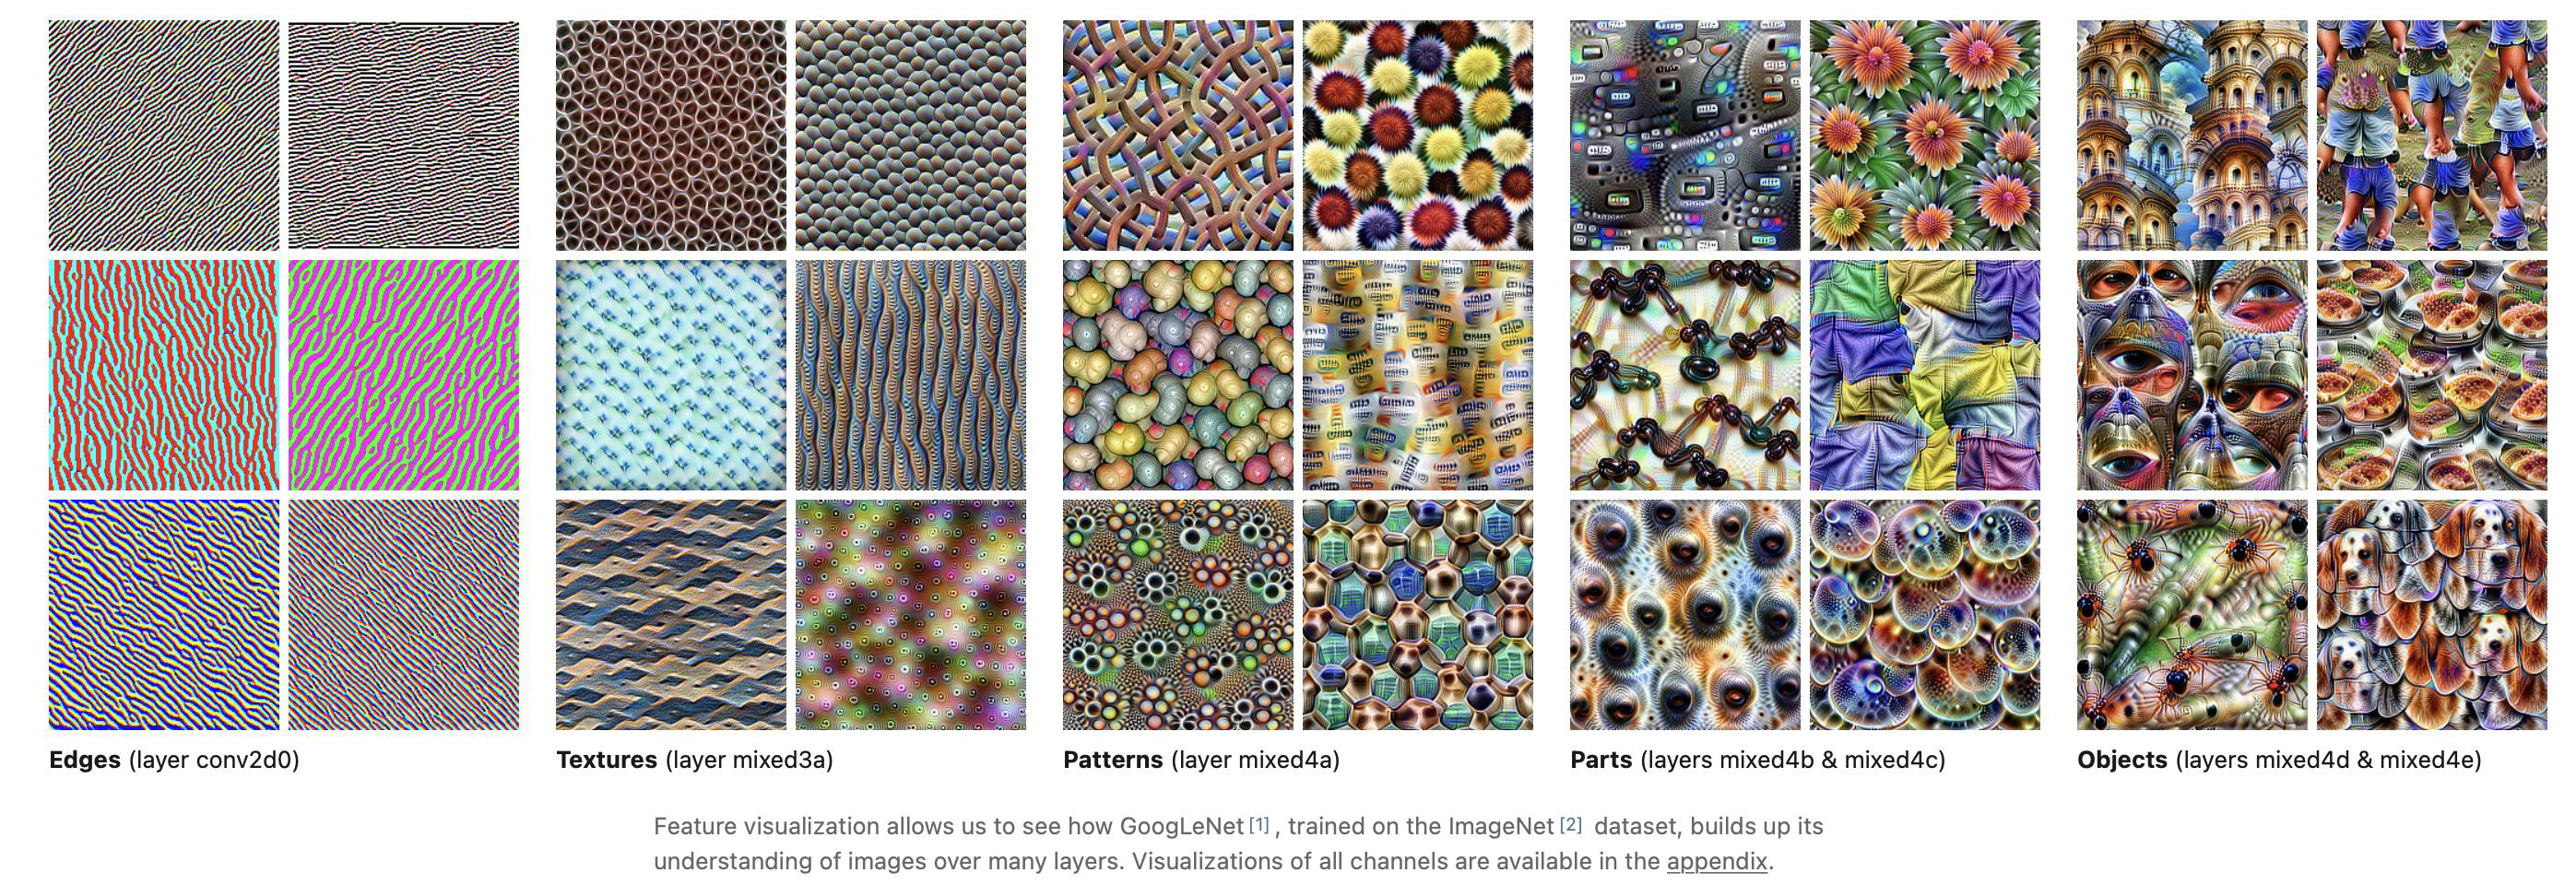
\includegraphics[width=1\linewidth]{images/week_4/visualising features 4.png}
    \caption{Progression from textures to object parts to full objects.}
    \label{fig:features-4}
\end{figure}

\subsection{Visualisation Techniques}

\begin{rigour}[Feature Visualisation via Optimisation]
To visualise what maximally activates a neuron/channel/class:
\begin{enumerate}
    \item Start with random noise image $X$
    \item Compute activation of target unit: $a = f(X)_{\text{target}}$
    \item Compute gradient: $\frac{\partial a}{\partial X}$
    \item Update image: $X \leftarrow X + \eta \frac{\partial a}{\partial X}$
    \item Repeat, possibly with regularisation (e.g., blur, $L_2$ penalty on $X$)
\end{enumerate}

The result shows the ``ideal'' input pattern for that unit.
\end{rigour}

\begin{quickref}[Feature Visualisation Methods]
\begin{enumerate}
    \item \textbf{Neuron visualisation}: Generate image that maximally activates a specific neuron
    \item \textbf{Channel visualisation}: Optimise for entire feature map to see what the filter detects
    \item \textbf{Layer visualisation} (DeepDream): Amplify patterns across a whole layer
    \item \textbf{Class visualisation}: Generate image that maximises a class probability
    \item \textbf{Gradient-weighted Class Activation Maps (Grad-CAM)}: Highlight which regions contribute to a classification decision
\end{enumerate}
\end{quickref}

\begin{quickref}[Why Visualisation Matters]
\begin{itemize}
    \item \textbf{Interpretability}: Understand what the network actually learns
    \item \textbf{Debugging}: Identify unexpected or biased features (e.g., detecting watermarks instead of objects)
    \item \textbf{Trust}: Critical for safety-sensitive applications (medical, autonomous driving)
    \item \textbf{Research}: Insights into representation learning and network behaviour
\end{itemize}
\end{quickref}

%==============================================================================
\section{Summary: CNN Building Blocks}
\label{sec:summary}
%==============================================================================

\begin{quickref}[CNN Layer Types]
\begin{center}
\begin{tabular}{llll}
\toprule
Layer & Purpose & Parameters & Key Property \\
\midrule
Convolution & Feature detection & $C_{\text{out}} \times C_{\text{in}} \times r^2$ & Equivariant \\
Pooling & Downsampling & 0 & Local invariance \\
Batch Norm & Normalisation & $2 \times C$ & Stabilises training \\
ReLU & Non-linearity & 0 & Sparse activation \\
Fully Connected & Classification & $H_{\text{in}} \times H_{\text{out}}$ & Dense \\
\bottomrule
\end{tabular}
\end{center}
\end{quickref}

\begin{quickref}[Key Formulas]
\textbf{Output dimension:}
\[
\text{Output} = \left\lfloor \frac{\text{Input} + 2P - r}{S} \right\rfloor + 1
\]

\textbf{Receptive field} (stride 1, same kernel size $r$, $L$ layers):
\[
\text{RF} = L(r - 1) + 1
\]

\textbf{Parameter count} (conv layer):
\[
\text{Params} = C_{\text{out}} \times (C_{\text{in}} \times r^2 + 1)
\]

\textbf{Backprop through conv:}
\[
\frac{\partial L}{\partial W} = X \star \delta, \quad \frac{\partial L}{\partial X} = \delta *_{\text{full}} \text{rot}_{180}(W)
\]
\end{quickref}

\begin{quickref}[Design Checklist]
\begin{itemize}
    \item[$\square$] Use $3 \times 3$ filters (or stack them for larger RF)
    \item[$\square$] Double channels when halving spatial dimensions
    \item[$\square$] Use batch normalisation after convolutions
    \item[$\square$] Consider strided convolutions instead of pooling
    \item[$\square$] Use global average pooling before final FC layer
    \item[$\square$] Apply data augmentation for images
    \item[$\square$] Ensure receptive field is large enough for target objects
\end{itemize}
\end{quickref}
